% ****** Start of file apssamp.tex ******
%
%   This file is part of the APS files in the REVTeX 4.1 distribution.
%   Version 4.1r of REVTeX, August 2010
%
%   Copyright (c) 2009, 2010 The American Physical Society.
%
%   See the REVTeX 4 README file for restrictions and more information.
%
% TeX'ing this file requires that you have AMS-LaTeX 2.0 installed
% as well as the rest of the prerequisites for REVTeX 4.1
%
% See the REVTeX 4 README file
% It also requires running BibTeX. The commands are as follows:
%
%  1)  latex apssamp.tex
%  2)  bibtex apssamp
%  3)  latex apssamp.tex
%  4)  latex apssamp.tex
%
\documentclass[%
 reprint,
%superscriptaddress,
%groupedaddress,
%unsortedaddress,
%runinaddress,
%frontmatterverbose,
%preprint,
%showpacs,preprintnumbers,
%nofootinbib,
%nobibnotes,
%bibnotes,
amsmath,amssymb,
%aps,
pra,
%prb,
%rmp,
%prstab,
%prstper,
%floatfix,
]{revtex4-1}

\usepackage{tabularx}
\usepackage{siunitx}
\usepackage{graphicx}% Include figure files
\usepackage{dcolumn}% Align table columns on decimal point
\usepackage{bm}% bold math
%\usepackage{hyperref}% add hypertext capabilities
%\usepackage[mathlines]{lineno}% Enable numbering of text and display math
%\linenumbers\relax % Commence numbering lines

%\usepackage[showframe,%Uncomment any one of the following lines to test
%%scale=0.7, marginratio={1:1, 2:3}, ignoreall,% default settings
%%text={7in,10in},centering,
%%margin=1.5in,
%%total={6.5in,8.75in}, top=1.2in, left=0.9in, includefoot,
%%height=10in,a5paper,hmargin={3cm,0.8in},
%]{geometry}

\begin{document}

\preprint{APS/123-QED}

\title{Fabrication and characterization of a Pseudo-MOSFET}% Force line breaks with \\

\author{Moritz Berger}
 \altaffiliation[]{RWTH Aachen University, Germany}%Lines break automatically or can be forced with \\
 \email{moritz.berger@rwth-aachen.de}
 \author{Gerald Kolter}
 \altaffiliation[]{RWTH Aachen University, Germany}%Lines break automatically or can be forced with \\
 \email{gerald.kolter@rwth-aachen.de}

%\date{May 1, 2019}
\date{\today}% It is always \today, today,
             %  but any date may be explicitly specified

\begin{abstract}
Pseudo-MOSFET structures have been investigated in recent years as they provide multiple applications. Additionally they can be used to determine relatively easily the charge carrier mobility $\mu _{eff}$ of different materials such as Si even in different configurations. In this paper a deeper look is given into important technologies used for fabricating Pseudo-MOSFETs, namely Optical Lithography and Reactive Ion Etching. Afterwards a set of devices is analyzed to characterize the output and transfer of the device, which give an indication of the quality of the device.
\end{abstract}

\maketitle


\section{Introduction}
The Pseudo-MOSFET structure is a simple test structure to determine properties of silicon film and silicon oxide \citep{Park}. \\
In the following the fabrication of a metallic-oxide-semiconductor-field-effect-transistor ("MOSFET") more precisely a Pseudo-MOSFET will be described. The next step is a more detailed description of optical lithographie and reactive ion etching. Afterwards an analysis and a discussion of the characterization of the fabricated Pseudo-MOSFET will be given. \\
The classical MOSFET structure consists of a silicon substrat on which a thin mesa structured layer of oxid with the metallic gate layer on top. A Semiconductor On Insulator ("SOI") MOSFET is essentially a MOSFET in which the silicon substrat is replaced with a SOI substrat which consists of a buried oxide layer in between a top-Si and a bulk-Si layer. The idea of the	$\Phi$-MOSFET is to take advantage of the configuration of SOI material where the buried oxide is used as the actual gate oxide and the silicon handle wafer as the gate electrode. \citep{Anleitung}


\section{Fabrication}
The basis for the MOSFET are SOI samples, the specifications are listed in table \ref{tab:Spec_SOI}. Si is used as semiconductor and SiO$_2$ as insulator. \\
In a first step, a mask for the mesa structuring was defined lithographically. The etching is done by reactive ion etching with a gas mixture of SF$_6$/O$_2$. For removing the resist, an oxygen plasma is used. At next the samples are RCA-cleaned ending with a dip in hydroflourid acid to get a bare silicon surface. \SI{100}{nm} aluminum is evaporated in a vacuum chamber. The aluminum layer is structured with optical lithographie and an aluminum wet etch. The used resist, developer, etchant and the energy deposition are listed in table \ref{tab:Spec_Fab_Al}.

\begin{table}[h]
\centering
\begin{tabular}{|c|c|}
\hline 
Fabrication technology & "UNIBOND" \\ 
\hline 
top Si thickness & \SI{85}{nm} \\ 
\hline 
buried oxide thickness & \SI{145}{nm} \\ 
\hline 
doping type & p-type (Boron) \\ 
\hline 
doping concentration & $1 \times 10^{15}$ \si{\per\cubic\centi\meter} \\ 
\hline 
crystal orientation & (100) \\ 
\hline 
\end{tabular} 
\caption{Specification of the SOI wafer.}
\label{tab:Spec_SOI}
\end{table}

\begin{table}[h]
\centering
\begin{tabular}{|c|c|}
\hline 
etchant & phosphoric acid, nitric acid, acetic acid and \\ 
 & water in a volume ratio of 16:1:1:2 \\ 
\hline 
resist & AZ5214F \\ 
\hline 
resist remover & aceton, isopropyl alcohol \\ 
\hline 
developer & AZ 726 MIF \\ 
\hline 
energy deposition & \SI{113.1}{mJ \per\centi\meter\square} @\SI{405}{nm} \\ 
\hline 
\end{tabular} 
\caption{Specification of the lithographie used for structuring the aluminum layer.}
\label{tab:Spec_Fab_Al}
\end{table}
\section{Theory}

\subsection{Optical Lithographie}

\begin{figure}
\centering
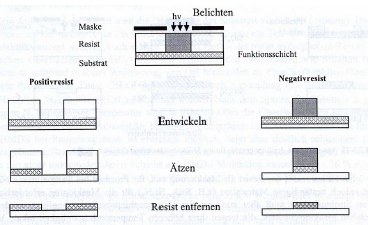
\includegraphics[scale=1.0]{Bilder/Lithographie.PNG}
\caption{Operating principle of Optical Lithographie with the different steps. Taken from \cite{Volklein00}}
\label{fig:Lithographie}
\end{figure}

The goal of optical lithographie is to build small structures of thin layers. In general, one distinguishes between two types of optical lithographie: Positiv (on the left in Fig. \ref{fig:Lithographie}) and negativ (on the right in Fig. \ref{fig:Lithographie}). \\
For both types the first step is to put a resist on the sample. The sample is spin-coated to get an evenly thin layer of resist at about \SI{1}{\mu m}. Afterwards the resist has to be baked. The next step is the exposure of the resist with a mask which defines the structure to be build. To remove the resist only at the relevant parts the sample is developed. At this step the difference between positiv and negativ lithographie can be seen the first time: In positiv lithographie the resist at the exposed parts is removed and in negativ lithographie the resist at the non-exposed parts is removed. \\
Afterwards the etching is applied and the resist prevents the layer underneath. As last step the remaining resist is removed with a dip into the resist remover.


\subsection{Reactive Ion Etching}

\begin{figure}
\centering
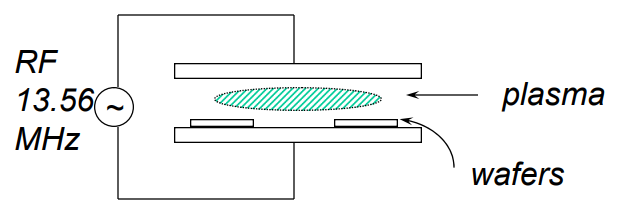
\includegraphics[scale=0.5]{Bilder/Reactive_Ion_Etching.PNG}
\caption{Setup for Reactive Ion Etching. Taken from \cite{Cheung}}
\label{fig:Reactive_Ion_Etching}
\end{figure}

The general setup for reactive ion etching is shown in fig. \ref{fig:Reactive_Ion_Etching}: In a vacuum chamber a capacitor with an oszillating electric field is placed. The sample gets placed on one electrode. The frequency used is $f = \SI{13.56}{MHz}$. The reason is to not get interference with frequencies used for radio outside the laboratory. \\
After the vacuum has established the etching gas is injected in the chamber. The fast oszillating strong electric field establishes a plasma separating the electrons and ions of the etching gas. In this plasma there are amoung others radicals (F*, O*) and positive (SF$_5^+$) and negative ions (F$^-$). These ions react with the silicon to be etched \cite{Jansen_1996}:
\begin{equation*}
\text{Si} + x \text{F*} \rightarrow \text{SiF}_x \qquad \text{with} \qquad x \leq 4
\end{equation*}
Siliconflourid is a gas and will be taken out of the vacuum chamber after the process. The radicals can react with the silicon, too \cite{Jansen_1996}: 
\begin{equation*}
\text{Si} + x \text{F*} + y \text{O*} \rightarrow \text{SiF}_x \text{O}_y
\end{equation*}
After the reactive ion etching an O$_2$ plasma is used to remove the resist.


\section{Measurement}
On the sample are multiple devices with different sizes. For one of these the output characteristic is measured via measuring the drain source current for different gate voltages depending on constant drain source voltage. \\
Afterwards the transfer characteristic is measured for multiple devices. This is done by measuring the drain source current for different gate voltages at constant drain voltage.\\
In figure \ref{fig:bezeichnung} an overview of the mesa structure is given. The quadrants are numbered from top left to bottom right.\\
During the measurement a lot of devices showed a drain-current that was significantly higher than expected (by a factor $10^5$). This indicates that these devices are short-circuited and unusable for measurement.

\begin{figure}
\centering
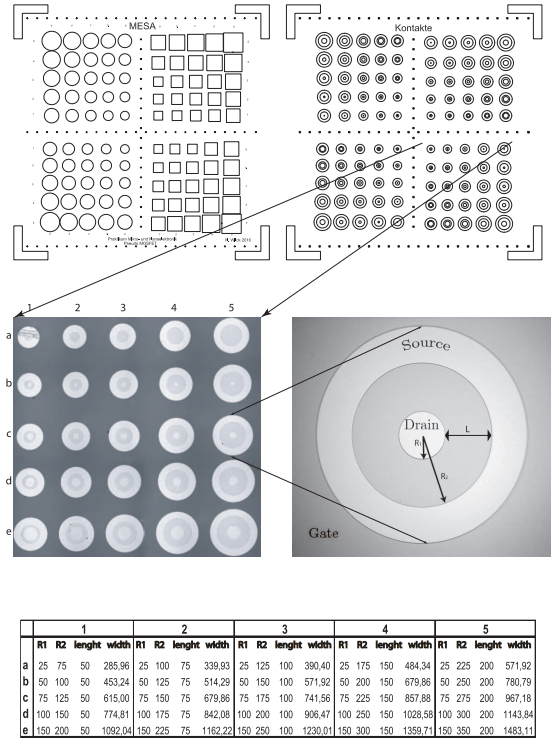
\includegraphics[scale=0.6]{Bilder/Screenshot_1.png}
\caption{Output curves for different gate-voltages.\cite{Anleitung}}
\label{fig:bezeichnung}
\end{figure}

\section{Data Analysis}
In the following chapter the characteristic values of the MOSFETs are extracted out of the measurement data. The methods that are used to do this are shown with the help of the data set of device A5 of the lower right quadrant (4-A5). This device has a tunnel length of \SI{200}{\mu m} with an inner radius of \SI{25}{\mu m} and an outer radius of \SI{225}{\mu m}.
\subsection{Output Characteristics}
\begin{figure}
\centering
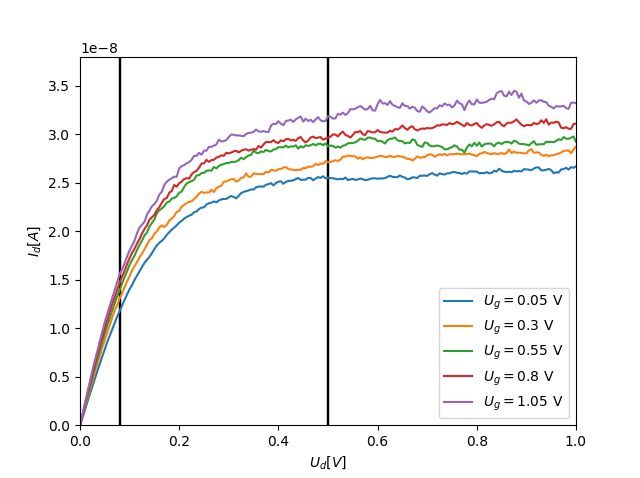
\includegraphics[scale=0.55]{Bilder/output.png}
\caption{Output curves for different gate-voltages. The first vertical line approximately indicates the end of the linear regime and the second the start of the saturation.}
\label{fig:output}
\end{figure}

In a first step the output characteristics of the device was measured to determine an appropriate gate voltage. For this the drain-voltage  $V_d$ was plotted against the drain-current $I_d$. As predicted by theoretical calculations the curves show a linear behavior for small drain-voltages. For the measured device and gate-voltages this goes up to approximately $V_d \approx \SI{0.08}{V}$. They enter saturation at around $V_d \approx \SI{0.5}{V}$. As a result of this three drain-voltages in the linear regime ($V_d = \SI{0.03}{V},\SI{0.05}{V} $ and \SI{0.07}{V}) were chosen and the transfer-characteristic was measured for each of these values.

\subsection{Transfer Characteristic}
\subsubsection{Effective Charge Carrier Mobility}
For the extraction of the effective charge carrier mobility $\mu_{eff}$ the $\frac{I_d}{\sqrt{g_m}}$-method is used.\\
First the measured drain-current $I_d$ is plotted against the gate-voltage $V_g$ for three different drain-voltages $V_d$ = \SI{0.03}{V}, \SI{0.05}{V} and \SI{0.07}{V} , as seen in figure \ref{fig:linreg1}. Then the point with the highest slope is determined numerically and a linear regression is fitted at a \SI{1}{\volt} area around this point. The resulting straights are also shown in figure \ref{fig:linreg1}.
\begin{figure}[h]
\centering
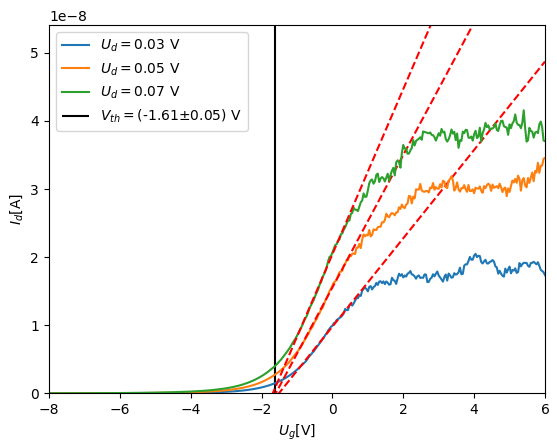
\includegraphics[scale=0.55]{Bilder/linreg.png}
\caption{Drain-current $I_d$ plotted against the gate-voltage $V_g$ for different drain Voltages. A linear fit is fitted against each curve.}
\label{fig:linreg1}
\end{figure}

The threshold-voltage $V_{th}$, as well as its error, can directly be extracted from this fit. This is done for all three curves and a final value for $V_{th}$ for this device is calculated by taking the weighted average of all three values.\\
\\
The slope of this fit is also used to determine $\mu_{eff}$ with the help of the following equation:
\begin{equation}
\sqrt{\mu_{eff} f C_{ox} V_d} \cdot (V_g-V_{th}) = \dfrac{I_d}{\sqrt{g}}
\end{equation}

where $f = \frac{2\pi}{ln(R_2/R_1)}$ is a structural factor, $C_{ox} = \epsilon_0 \epsilon_{ox} / d_{ox}$ is the capacity of the oxide-layer and g is the slope. $\epsilon_{ox} = 3.9$ is used. A constant error of \SI{0.1}{\mu m} is assumed for the radii $R_1$ and $R_2$ to account for uncertainties in the fabrication process.\\
In order to determine  $\mu_{eff}$ the right side of this equation $I_d/\sqrt{g}$ is plotted against $V_g$, as seen in figure \ref{fig:linreg2}. This figure displays $I_d/\sqrt{g}$ plotted against $V_g \cdot \sqrt{V_d}$ in order to compare the three slopes without the differing influence of $V_d$. A second linear regression is then fitted to the data. From the slope $a$ of this fit one can get $\mu_{eff}$ through the following equation:
\begin{equation}
\mu_{eff} = \dfrac{a^2}{f C V_d}
\end{equation}
This is also done for all three drain-voltages. A final value for $\mu_{eff}$ is again calculated by taking the weighted average. The results are listed in table \ref{tab:exaple_data}.
\begin{figure}
\centering
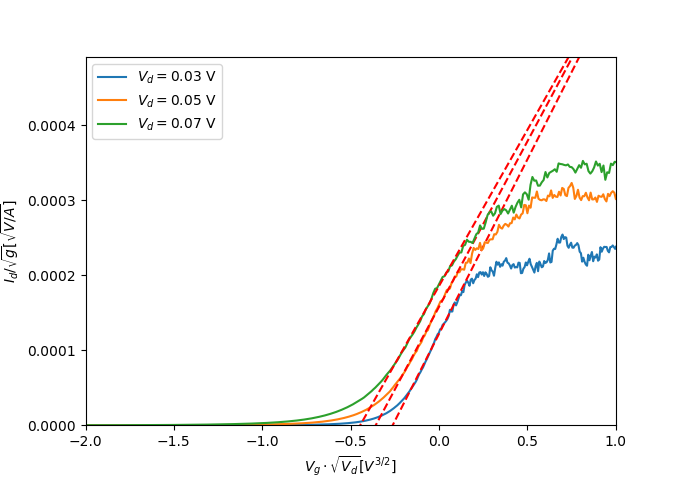
\includegraphics[scale=0.55]{Bilder/mu.png}
\caption{$I_d/\sqrt{g}$ plotted against $V_g \cdot \sqrt{V_d}$ for different drain voltages, including the second linear fit to determine $\mu_{eff}$.}
\label{fig:linreg2}
\end{figure}
\begin{table}
\centering
\begin{tabular}{|c|c|c|c|}
\hline
$U_d$ & $V_{th}[\si{V}]$ & $g[\si{nA/V}]$ & $mu_{eff}[\si{cm^2/Vs}]$\\
\hline
0.03 & $-1.51\pm 0.02$ & $6.48\pm 0.07$ & $0.59\pm 0.02$\\
\hline
0.05 & $-1.6\pm 0.02$ & $9.72\pm 0.09$ & $0.53\pm 0.01$\\
\hline
0.07 & $-1.69\pm 0.02$ & $12.12\pm 0.1$ & $0.47\pm 0.01$\\
\hline
average & $-1.61\pm 0.05$ & $8.64\pm 1.6$ &$0.51\pm 0.03$\\
\hline
\end{tabular}
\caption{Results for device 4-A5.}
\label{tab:exaple_data}
\end{table}





\subsubsection{Subthreshold-Slope}

The subthreshold slope is an important characteristic of a MOSFET because it gives an indication for how fast it can change its behavior. A steeper slope means that a smaller voltage difference is required for it to be turned on, which can be achieved quicker. A perfect MOSFET would have an infinite slope which corresponds to a step-function characteristic.\\
\\
In order to analyze the subthreshold slope the drain-current is plotted logarithmicly against the gate-voltage as shown in figure \ref{fig:log}. A voltage area is then manually  selected, in which the curves appear to be linear. In this area a linear fit is fitted against the curves in order to obtain the slope. Because the subthreshold slope is usually given by the unit $\si{V/dec}$ the final value is obtained by
\begin{equation}
\Delta V = \dfrac{log(10)}{a}
\end{equation}
where $a$ denotes the initial slope.\\
For the example device the voltage for the fit ranges from \SI{-8}{V} to \SI{-4.5}{V}. The results of this are shown in table \ref{tab:subthreshold_example}.

\begin{table}[h]
\centering
\begin{tabular}{|c|c|c|}
\hline
$U_d$[\si{V}] & a [log(A)/V] & subthreshold-slope [V/dec] \\
\hline
0.03 & $0.71\pm 0.02$ & $3.26\pm 0.10$\\
\hline
0.05 & $0.74\pm 0.03$ & $3.13\pm 0.11$\\
\hline
0.07 & $0.75\pm 0.03$ & $3.06\pm 0.11$\\
\hline
average & $0.73\pm 0.02$ & $3.16\pm 0.09$\\
\hline
\end{tabular}
\caption{Results of the subthreshold analysis.}
\label{tab:subthreshold_example}
\end{table}

\begin{figure}[h]
\centering
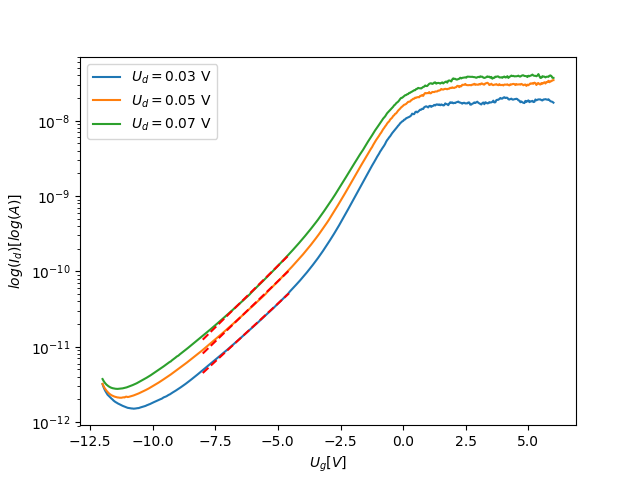
\includegraphics[scale=0.55]{Bilder/log.png}
\caption{$\log(I_d)$ plotted against $V_g$ for different drain Voltages to analyze the subthreshold slope.}
\label{fig:log}
\end{figure}



\subsubsection{Ambipolarity}
The curve that was analyzed until now shows a current flow for increasing gate-voltages. This corresponds to electrons moving through the device. However for certain devices there also exists a current flow for decreasing gate-voltages, as shown in figure \ref{fig:ambipol} for device 4-C3. This can be explained by the fact that (positively charged) electron-holes can move through the device for negative gate-voltages. This phenomenon is called ambipolarity.

\begin{figure}
\centering
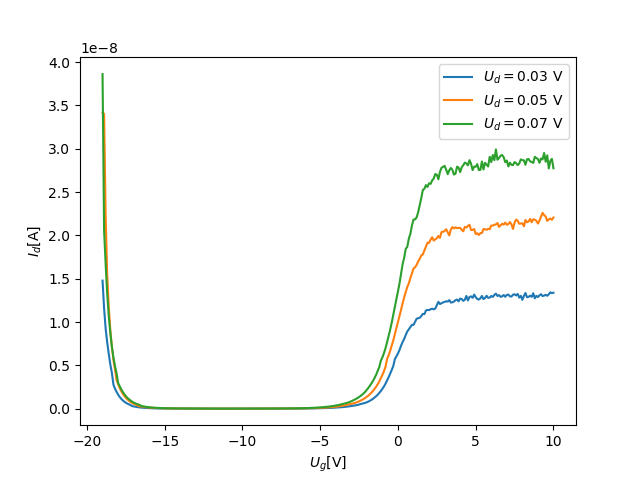
\includegraphics[scale=0.6]{Bilder/amipol.png}
\caption{transfer characteristic of device 4-C3 for the full negative range of $V_g$. A second current flow can be observed for large negative voltages.}
\label{fig:ambipol}
\end{figure}


\section{Results and Discussion}
The analysis described in the previous chapter is done for all measured devices. The results are listed in table \ref{tab:transfer_results}.\\
In order to have a better overview over the data $\mu_{eff}$ is plotted against the channel-length, as seen in figure \ref{fig:plot}. It turns out that a lot of devices have a rather small mobility, while other have one that up to 2 orders larger. This even occurs for devices with the same channel length and does not seem to be related to the size of the device at all. This makes an analysis of the channel-length dependence impossible.\\
However this phenomenon seems to have a correlation with the threshold- voltage. For small $\mu_{eff}$ the threshold-voltage also seems to be small (larger negative values). This indicates that the devices are influenced by something that is not wanted, most likely fabrication related. It could be that the contact between aluminum and silicon is not perfect, because the SOI was not perfectly cleaned. As a result the Schottky-barriers would be imperfect and have a different current flow behavior. The fact that the aluminum layer was also not perfectly removed further indicates that there was a problem with the fabrication.
\begin{figure}
\centering
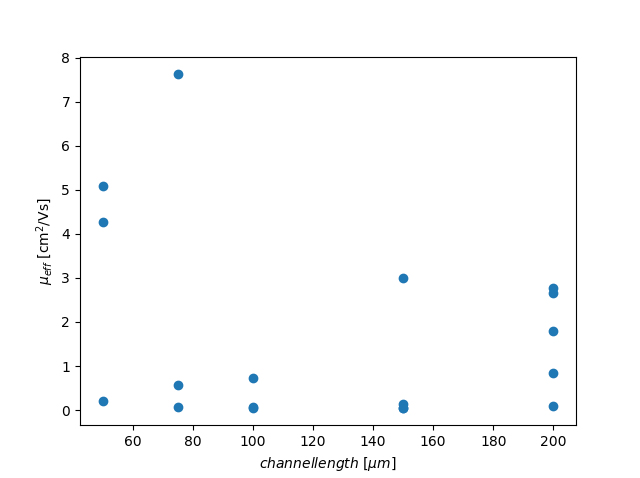
\includegraphics[scale=0.55]{Bilder/figure_1.png}
\caption{Charge carrier mobility plotted against the channel length.}
\label{fig:plot}
\end{figure}
Literature values for Pseudo-Mosfets are usually of the order of \SI{100}{cm^2/Vs}, for example in \cite{Loss98} the carrier mobility is 250-\SI{360}{cm^2/Vs}. This means that even the mobility of the correctly functioning devices are smaller by a factor 100 when compared to literature values. One of the reasons for this can be in the use of different materials or structure. The measurements of the SOI might not be optimized to deliver a high mobility. The materials can also influence the height of the Schottky barriers and therefore the mobility.\\
\\
The subthreshold-slope values are also listed in table \ref{tab:transfer_results}. Please note that for the devices 4-E2, 4-E3 and 4-E4 the slope was mostly nonlinear, which resulted in a higher value. The other slopes vary between 2-\SI{4}{V/dec}. This is also higher and therefore worse than comparable literature values, which are usually smaller than \SI{1}{V/dec} (\cite{Loss98}, \cite{mos}). This has similar reasons to the ones listed above.
\newpage



\begin{table}
\centering
\begin{tabular}{|c|c|c|c|c|c|c|}
\hline 
Position & length & $R_1$ & $R_2$ & $V_{th}$ [\si{\volt}]  & $\mu_{eff}$  [\si{cm^2/Vs}] & $\Delta V$ [\si{V/dec}]\\ 
\hline 
4-a1 & 50 & 25 & 75 & $-2.63\pm 0.14$ & $0.21\pm 0.03$ & $1.93\pm 0.07$\\
\hline 
3-d1 & 50 & 50 & 100 & $-1.28\pm 0.01$ & $5.09\pm 0.07$& $2.1\pm 0.11$\\
\hline 
3-e1 & 50 & 150 & 200 & $-0.61\pm 0.01$ & $4.27\pm 0.01$& $3.07\pm 0.09$\\
\hline 
\hline 
1-b2 & 75 & 50 & 125 & $-0.54\pm 0.02$ & $7.62\pm 0.22$& $2.68\pm 0.1$\\
\hline 
1-d2 & 75 & 100 & 175 & $-4.29\pm 0.35$ & $0.07\pm 0.01$& $3.33\pm 0.05$\\
\hline 
4-e2 & 75 & 150 & 225 & $1.31\pm 0.17$ & $0.57\pm 0.04$& $6.28\pm 0.32$\\
\hline 
\hline  
4-b3 & 100 & 50 & 150 & $-4.03\pm 0.05$ & $0.08\pm 0.01$& $3.06\pm 0.05$\\
\hline 
4-c3 & 100 & 75 & 175 & $-1.51\pm 0.01$ & $0.72\pm 0.02$& $2.65\pm 0.13$\\
\hline 
4-e3 & 100 & 150 & 250 & $-3.41\pm 2.08$ & $0.04\pm 0.01$& $8.85\pm 0.18$\\
\hline
\hline 
4-b4 & 150 & 50 & 200 & $-4.9\pm 0.24$ & $0.04\pm 0.01$& $3.22\pm 0.05$\\
\hline
4-c4 & 150 & 75 & 225 & $0.25\pm 0.01$ & $3.0\pm 0.08$& $4.22\pm 0.22$\\
\hline 
4-d4 & 150 & 100 & 250 & $-4.08\pm 0.08$ & $0.13\pm 0.01$& $3.16\pm 0.05$\\
\hline 
4-e4 & 150 & 150 & 300 & $-5.34\pm 1.73$ & $0.04\pm 0.01$& $10.76\pm 0.39$\\
\hline 
\hline 
4-a5 & 200 & 25 & 225 & $-1.61\pm 0.05$ & $2.77\pm 0.17$& $3.16\pm 0.09$\\
\hline 
4-b5 & 200 & 50 & 250 & $-2.34\pm 0.02$ & $0.85\pm 0.03$& $3.04\pm 0.05$\\
\hline 
4-c5 & 200 & 75 & 275 & $-3.19\pm 0.22$ & $0.09\pm 0.02$& $4.72\pm 0.28$\\
\hline
4-d5 & 200 & 100 & 300 & $-1.21\pm 0.02$ & $2.65\pm 0.03$& $2.8\pm 0.03$\\
\hline 
4-e5 & 200 & 150 & 350 & $-1.56\pm 0.06$ & $1.79\pm 0.1$& $2.69\pm 0.05$\\
\hline 
\end{tabular} 
\caption{Results of transfer characterization. The Position of the corresponding device is denoted by [quadrant-gridposition]. $\Delta V$ denotes the subthreshold-slope.}
\label{tab:transfer_results}
\end{table}
\section{Conclusion}
The fabricated and measured devices qualitatively behave like it was expected. The measurement of the output characteristic resulted in a linear behavior up to \SI{0.08}{V} and the reach of saturation at \SI{0.5}{V}.\\
\\
However due to problems in the fabrication a lot of devices did not work correctly which resulted in very low mobilities. As a consequence of this the influence of the channel length could not be analyzed.\\
Furthermore both the subthreshold and the mobilities suggest that the structure of the devices is unoptimized, because their characterization qualities are worse than other comparable devices.


\bibliography{MOSFET}% Produces the bibliography via BibTeX.

\end{document}
